\chapter{The Search for Gravitational Waves}

The field of ground-based gravitational-wave (GW) physics is rapidly
approaching a state with a high likelihood of detecting GWs for the
first time. Such a detection will not only validate part of Einstein's
general theory of relativity, but initiate an era of astrophysical
observation of the universe through GWs. Gravitational waves are
dynamical strains in space-time that travel at the speed of light and
are generated by non-axisymmetric acceleration of mass. The frequency
of the gravitational wave depends on its source. A first detection is
expected to witness an event such as a binary black
hole/neutron star merger. This chapter provides the theoretcial
framework of gravitational wave generation and presents various ways
to detect them, including the current status of an effort to do so.

\section{The theory of gravitational radiation}
Gravitational radiation is a perturbation $|h_{\mu \nu}|
\ll 1$ to the flat space-time Minkowski metric $\eta_{\mu \nu} =
\mbox{diag}(-1, 1, 1, 1)$. The metric describing space-time in the
presence of gravitational radiation is therefore
\begin{equation}
g_{\mu\nu} = \eta_{\mu\nu} + h_{\mu\nu}.
\end{equation}
Just as in electrodynamics where one has freedom in choosing the
vector potential $\vec{A}$ for calculating the magnetic field $\vec{B}
= \vec{\nabla} \times \vec{A}$, one also has freedom in general
relativity in choosing the form of $h_{\mu \nu}$ for ease of calculation. A
convenient and popular choice is called the transverse-traceless (TT)
gauge in which
\begin{equation}
h_{\mu \nu} = 
\left\llbracket \begin{array}{c c c c} 
0 & 0 & 0 & 0\\ 
0 & h_+ & h_\times & 0 \\
0 & h_\times & -h_+ & 0 \\
0 & 0 & 0 & 0
\end{array} \right\rrbracket
\end{equation}
where the $+$ and $\times$ represent two linearly independent
polarizations. Without loss of generality, we consider the $h_+$
polarization in the example that follows.

For a gravitational wave traveling along the $z$ axis, the metric is
given by:
\begin{equation}
ds^2 = -c^2dt^2 + [1+h_+(t)] dx^2 + [1-h_+(t)] dy^2.
\end{equation}
This says the TT coordinate system is stretched along the $x$ axis and
and compressed along the $y$ axis by a factor of 
\begin{equation}
\sqrt{1 \pm h_+(t)} \approx 1 \pm \frac{1}{2} h_+(t).
\label{eq:deltaL}
\end{equation}
Therefore, the \emph{proper distance} between two free masses located
along either the $x$ or the $y$ axes changes by the factor in
Eq. \ref{eq:deltaL}; their coordinate separations remain constant. The
GW perturbation is a dimensionless strain
\begin{equation}
h = 2 \frac{\Delta L}{L}.
\end{equation}



\section{Sources}
Any object with an accelerating mass quadrupole moment generates
gravitational waves. The typical strain amplitudes, however, are
extremely tiny: a binary system of coalescing $1 \mbox{M}_\odot$
neutron stars in the Virgo Cluster (a distance of 15 Mpc) would
produce a maximum GW strain on Earth of only
$10^{-21}$. \textcolor{blue}{Not right--fix this!!} The strain is
proportional to source mass and velocity, and inversely proportional
to distance from the observer:
\begin{equation}
h \approx \frac{GMv^2}{Rc^4}
\end{equation}
Consequently, the most promising sources of detectable gravitational
waves are nearby, fast-moving, massive astrophysical objects that
include
\begin{itemize}
\item supernovae \vspace{-10pt}
\item binary stars (orbiting or coalescing) \vspace{-10pt}
\item spinning neutron stars \vspace{-10pt}
\item cosmological/astrophysical background
\end{itemize}
and can be categorized as producing periodic, burst, or stochastic GWs.

Stably orbiting binary star systems comprised of black holes or
neutron stars as well as rapidly spinning non-axisymmetric pulsars are
considered periodic sources since they will produce GWs
of relatively constant frequency. These reliable sources of GWs
require a long integration time to pick out their signal above
noise. The Hulse-Taylor binary, for instance, falls into this
category. Supernovae are burst sources since the gravitational
collapse will produce a short-lived, unmodeled emission of
GWs. Binaries in their final tens of milliseconds of inspiral also
fall into this category. Finally, the anisotropies in the inflation of
the universe together with the hum of all distant astrophysical
sources will create a stochastic background of radiation. Coherent
cross-correlation between multiple detectors is necessary for
measuring the constant amplitude, broad-spectrum GW background.

Directly detecting gravitational radiation from any such source will
reveal information that electromagnetic radiation cannot convey. The
frequency of the GW tells about the dynamical timescale of the
source. Only through GW radiation, for example, can mass and spin
properties of a black hole be revealed.





\section{Methods of detection}
\begin{itemize}
\item Hulse/Taylor
\item Resonant bars
\item Pulsar timing
\item CMB polarization (B-modes)
\item Interferometry
\end{itemize}
For an approachable overview of the history of the field, including
detector design choices and estimated GW strain amplitudes of various
sources, refer to Ref. \cite{Linsay1983Study}.






\section{State of ground-based interferometry}
A network of first generation kilometer scale laser interferometer
gravitational-wave detectors completed its integrated 2-year data
collection run in 2007, called S5. The instruments were: the American
Laser Interferometer Gravitational-wave Observatories (LIGO)\cite{Abbott2009LIGO},
one in Livingston, LA with 4 km long arms and two in Hanford, WA with
4 km and 2 km long arms; the 3 km French-Italian detector
VIRGO\cite{Acernese2008Virgo} in Cascina, Italy; and the 1.2 km
German-British detector GEO\cite{Luck2006Status} in Ruthe, Germany. Multiple
separated detectors increase detection confidence through signal
coincidence and improve source localization through triangulation.

The first generation of LIGO, known as Initial LIGO, achieved its
design goal of sensitivity to GWs in the 40~Hz - 7000~Hz band which
included an impressive record strain sensitivity of
$2\times10^{-23}/\sqrt{\mathrm{Hz}}$ at 155~Hz. However, only the
loudest of sources produce enough GW strain to appear in LIGO's band,
and no gravitational wave has yet to be found in the S5 data. A second
generation of LIGO detectors, Advanced LIGO, has been designed to be
at least an order of magnitude more sensitive at several hundred Hz
and above and include an impressive increase in bandwidth down to
10~Hz, dramatically increasing the chances of detection. To test some
of Advanced LIGO's new technologies, an incremental upgrade to the
detectors was carried out after S5 \cite{Adhikari2006Enhanced}. This
project, Enhanced LIGO, culminated with the S6 science run from July
2009 to October 2010. Currently, construction of Advanced LIGO is
underway. VIRGO and GEO will both undergo their own upgrades as well
\cite{Acernese2008Virgo} \cite{Luck2010Upgrade}. See Figure
\ref{fig:h_all} for achieved and theoretical noise curves.

\begin{figure}
\begin{centering}
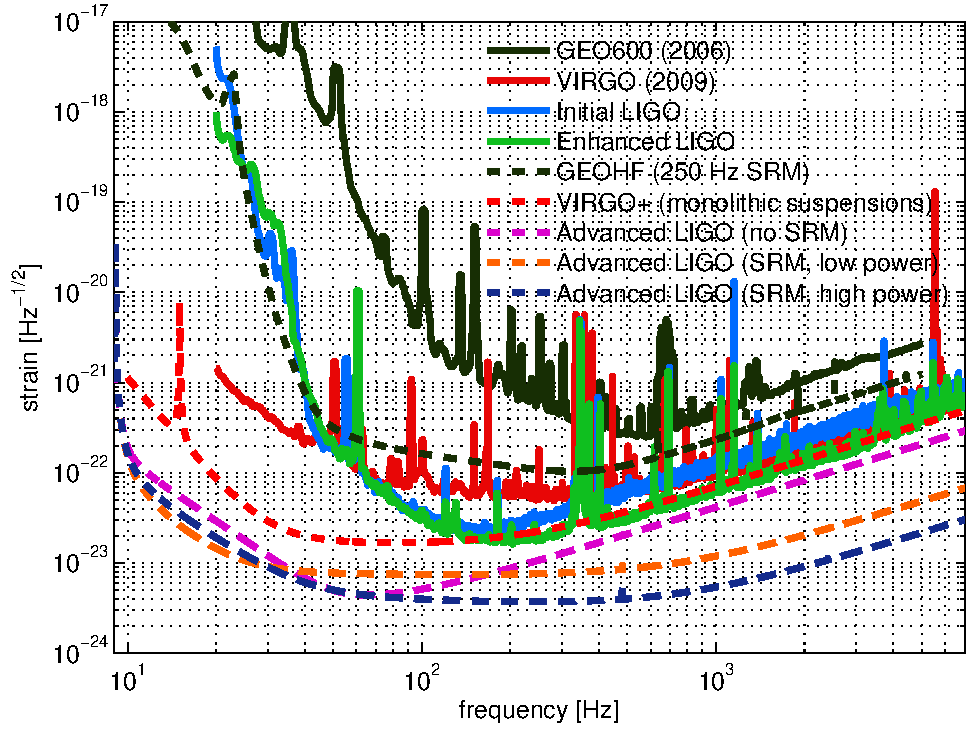
\includegraphics[width=1.0\textwidth]{figures/GWnetwork_strains.pdf}
\caption{Strain sensitivities of LIGO-VIRGO collaboration interferometers.}
\label{fig:h_all}
\end{centering}
\end{figure}

The baseline Advanced LIGO design \cite{AdvLigoSysDesign} improves
upon Initial LIGO by featuring better seismic isolation, the addition
of a signal extraction mirror at the output port, homodyne readout,
and an increase in laser power from 10~W to 200~W. The substantial
increase in laser power improves the shot-noise-limited sensitivity,
but introduces a host of radiation pressure and thermally induced side
effects that must be addressed for proper operation.

The recently completed Enhanced LIGO tested portions of the Advanced
LIGO designs so unforeseen difficulties could be addressed and so that
a more sensitive data taking run could take place. An output mode
cleaner was designed, built and installed, and DC readout of the GW
signal was implemented \cite{Fricke2011DC}. An Advanced LIGO active
seismic isolation table was also built, installed, and tested
\cite{KisselThesis}. In addition, the 10~W Initial LIGO laser was
replaced with a 35~W laser \cite{Frede2007Fundamental}. Accompanying
the increase in laser power, the test mass Thermal Compensation System
\citep{Willems2009Thermal}, the Alignment Sensing and Control, and the
Input Optics were modified. The upgrades of the latter two subsystems
make up the content of this dissertation.








